\documentclass{article}
\usepackage{graphicx}  % For including images
\usepackage{caption}   % For captions in figures
\usepackage{hyperref}  % For clickable references

\begin{document}
	
	\title{Analysis of Heart Disease Data}
	\author{Your Name}
	\date{\today}
	\maketitle
	
	\section*{Overview}
	In this report, we analyze various aspects of heart disease prevalence across different demographics and health metrics. The following plots illustrate our findings:
	
	\section{Gender and Heart Disease Distribution}
	Figure~\ref{fig:gender_heart_disease} shows the histogram of gender distribution among people diagnosed with heart disease. This allows us to visually compare the number of cases between males and females.
	
	\begin{figure}[h]
		\centering
		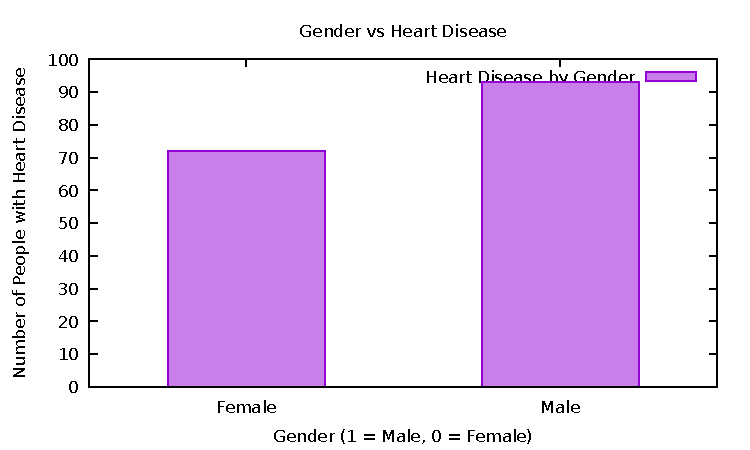
\includegraphics[width=0.6\textwidth]{a.pdf}
		\caption{Histogram of Gender vs. Number of People with Heart Disease}
		\label{fig:gender_heart_disease}
	\end{figure}
	
	\section{Correlation of Age with Health Metrics}
	
	\subsection{Age vs. Blood Pressure}
	Figure~\ref{fig:age_vs_bp} illustrates the correlation between age and blood pressure. Each point represents an individual case, highlighting any patterns that may emerge with aging.
	
	\begin{figure}[h]
		\centering
		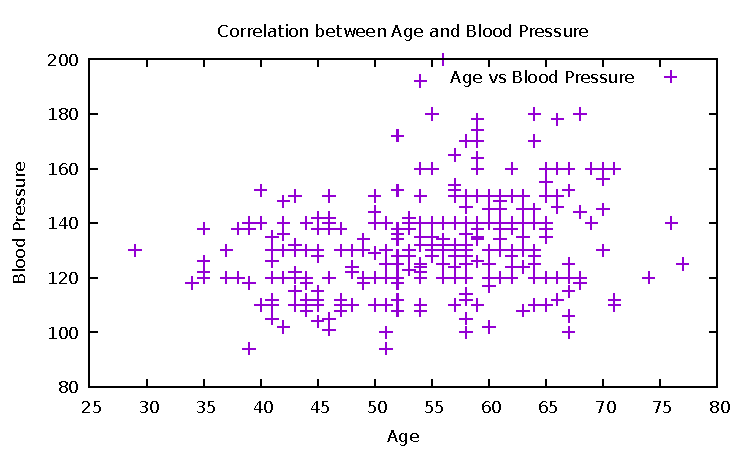
\includegraphics[width=0.6\textwidth]{b.pdf}
		\caption{Correlation between Age and Blood Pressure}
		\label{fig:age_vs_bp}
	\end{figure}
	
	\subsection{Age vs. Cholesterol for People Without Heart Disease}
	In Figure~\ref{fig:age_vs_chol}, we analyze the correlation between age and cholesterol levels specifically for individuals without heart disease. The line plot provides insight into cholesterol trends across different age groups.
	
	\begin{figure}[h]
		\centering
		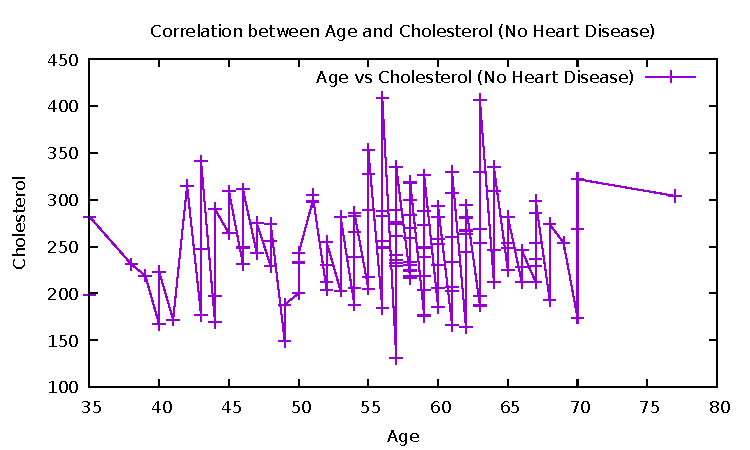
\includegraphics[width=0.6\textwidth]{c.pdf}
		\caption{Correlation between Age and Cholesterol (No Heart Disease)}
		\label{fig:age_vs_chol}
	\end{figure}
	
	\section{Age Group Distribution of Heart Disease Cases}
	Finally, Figure~\ref{fig:age_group_distribution} displays a pie chart representing the percentage of heart disease cases across different age groups, segmented into 10-year intervals from ages 40 to 100.
	
	\begin{figure}[h]
		\centering
		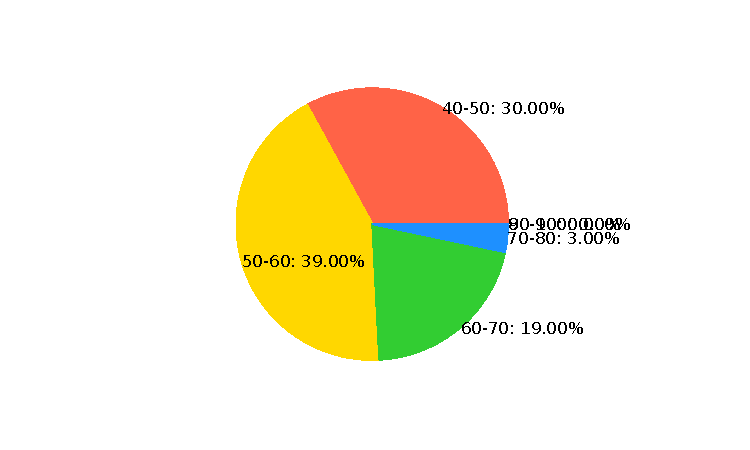
\includegraphics[width=0.6\textwidth]{d.pdf}
		\caption{Percentage of Heart Disease Cases by Age Group}
		\label{fig:age_group_distribution}
	\end{figure}
	
	\section*{Conclusion}
	The data visualizations above provide insights into the distribution and correlation of heart disease cases across gender, age, blood pressure, and cholesterol levels. Each of these figures offers a unique perspective on the factors associated with heart disease.
	
\end{document}
